\chapter{Performant Web Applications}%
\label{cha:performant_web_applications}

\minitoc%

\section{A Brief History of Native Code in the Client}%
\label{sec:native_client}

\begin{figure}[h]
	\centering
	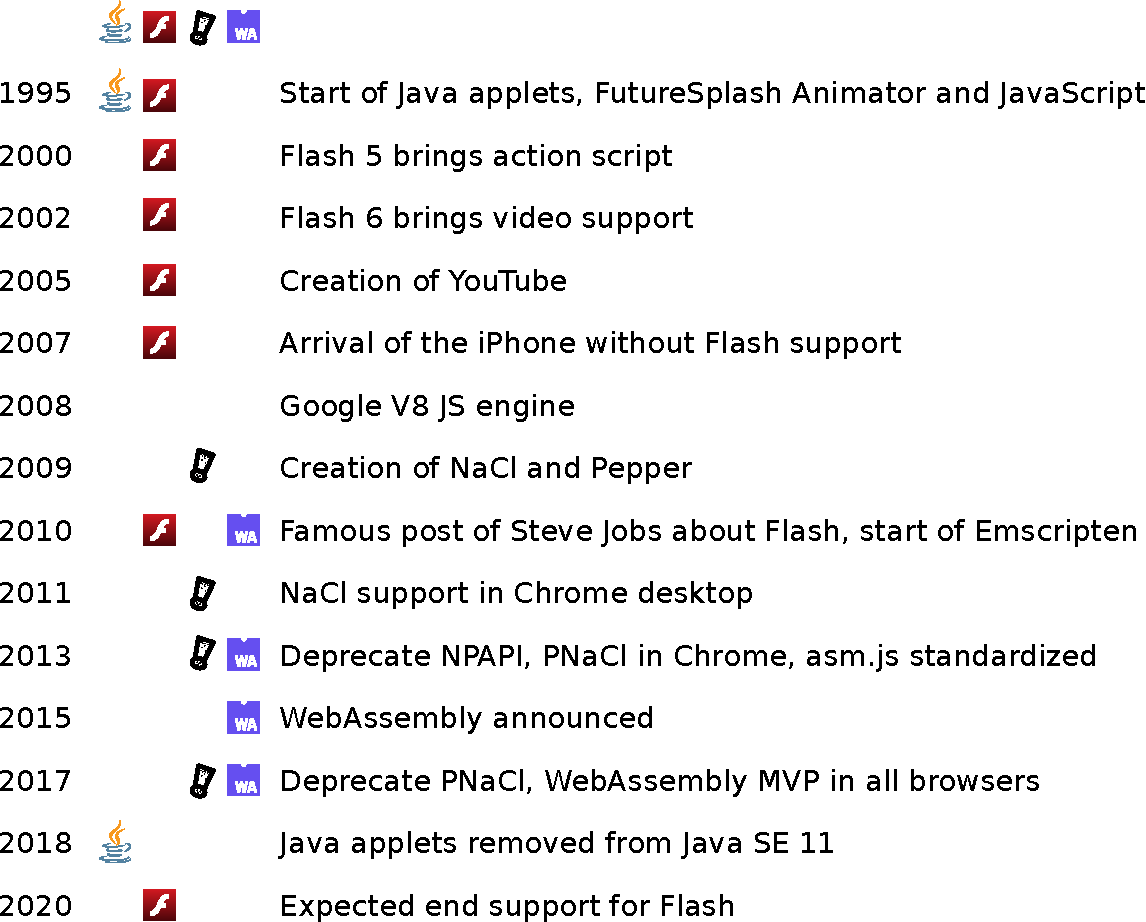
\includegraphics[width=\linewidth]{assets/img/wasm-timeline.pdf}
	\caption{Events releated to the birth and growth of WebAssembly.}%
	\label{fig:wasm-timeline}
\end{figure}

Being able to run high performance code in the browser
unlocks many use cases, including scientific computing.
Yet, it remains a challenging task.
Resources often refers to this as ``native'' code
but the terminology is rather vague.
Depending on the context, it may have one of the following meanings,
\begin{enumerate}
\setlength\itemsep{-0.5em}
	\item code statically compiled directly to the target architecture and running from the browser,
	\item code compiled from a typical ``native'' language such as C or C++,
	\item or anything that is not generating JavaScript.
\end{enumerate}
The distinction between those and how they relate to ``native'' code
will be made clearer after a brief history of high performance code in browsers.

\subsection{Java Applets}%
\label{sub:java_applets}

In 1995, just four years after the birth of the Web,
the Java programming language was created.
It appeared with a companion technology called Java Applet,
designed to run Java applications in the browser.
The Java Virtual Machine (JVM) was hosted by browsers,
enabling much better performances than JavaScript at this time.
As an example, Brendon C. Glazer worked on interactive ray tracing
of VRML scenes with Java applets in 1999~\cite{Glazer1999InteractiveRT}.
Figure~\ref{fig:glazer-thesis} depicts how the applet would appear
in a Web page at that time.
Since 1998 Java applets have also had access to 3D hardware acceleration~\cite{Java3dAPISpec}
whereas JavaScript waited until 2011 for WebGL in HTML5 canvas.

\begin{figure}[h!]
	\centering
	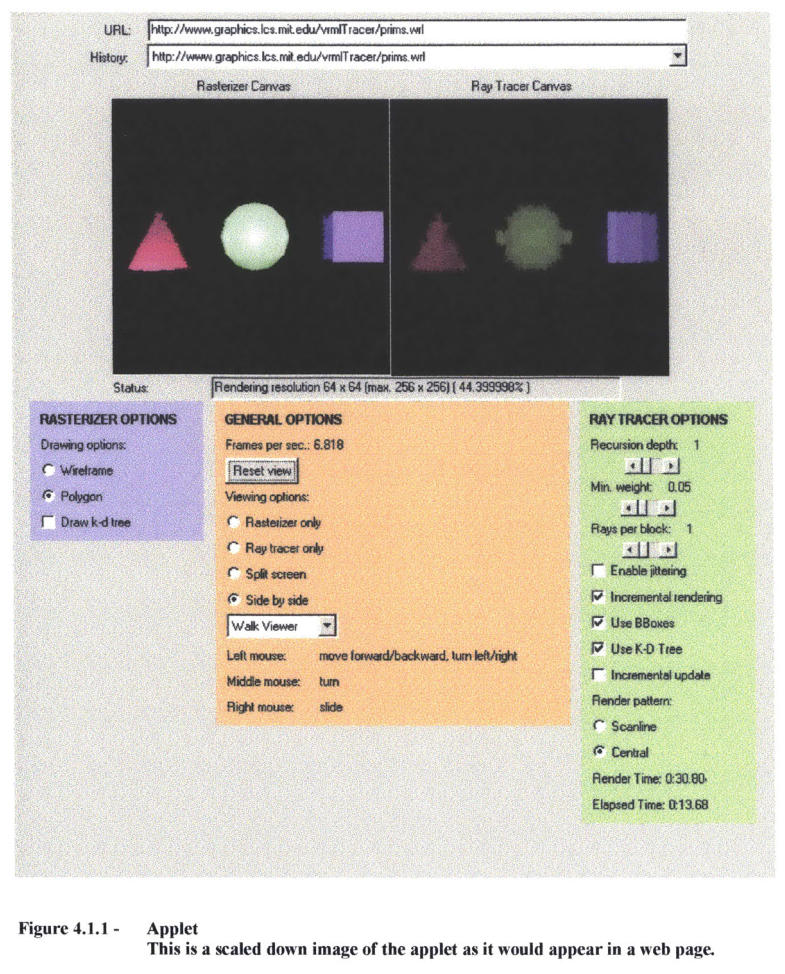
\includegraphics[width=\linewidth]{assets/img/glazer-thesis.jpg}
	\caption{Interactive ray tracing applet from Brendon C. Glazer master thesis (1999).}%
	\label{fig:glazer-thesis}
\end{figure}

On the down side, Java applets would break accessibility of the Web.
Screen readers would not be able to parse the content of the dedicated
applet area in the page.
The security model of Java applets was also quite risky.
Applets would have to get approved by a browser user and then gain rights
equivalent to a native application on your desktop.
Unfortunately, just like terms of service, most people just click ``agree''
and move on.
In addition, the Java Runtime Environment (JRE) has had hundreds security
vulnerabilities~\cite{JreCve} in its lifetime.
This represents a serious security threat for browser vendors.
Java applets were eventually entirely removed from Java SE 11, in 2018.

\subsection{Flash}%
\label{sub:Flash}

In his ``History of Flash''~\cite{HistoryFlash}, Jonathan Gay retraces the early days of Flash.
In 1993, he, Charlie Jackson and Michelle Welsh founded FutureWave Software
but their initial vector drawing application did not draw much attention (pun intended).
After discussions at Siggraph 1995, the company decided to focus on a web animation
product named ``FutureSplash Animator''.
It gained reputation with Microsoft and Disney using it and as a consequence,
was acquired by Macromedia and rebranded ``Flash'' in 1996.

Contrary to Java applets, Flash use cases started very narrow.
It provided a simple and efficient solution to build and share animations on the web,
giving a visual advantage over pure HTML documents.
In year 2000, Flash 5 was released, with the ActionScript programming language,
bringing even more potential to Flash-based websites.
Two years later, in 2002, Flash 6 brought support for real-time messaging protocols,
enabling video and audio streaming capabilities.
This represents roughly 8 years until 2010 when such capabilities are also
supported through HTML5 in most browsers.
In the meantime, highly influencial projects shaped the Web thanks to Flash.
You may have heard of Chad Hurley, Steve Chen and Jawed Karim who launched
YouTube in 2005, based on Flash.

In spite of the many advantages of Flash and ActionScript over classic Web pages,
it also had similar flaws than Java applets.
In October 2000, usability consultant Jakob Nielsen published a short article
entitled ``Flash: 99\% Bad''~\cite{FlashBadNielsen} stating that
``Flash technology tends to discourage usability for three reasons:
it makes bad design more likely,
it breaks with the Web's fundamental interaction style,
and it consumes resources that would be better spent enhancing a site's core value.''
Apple also played a huge role in Flash decline.
In 2007 the iPhone launched without Flash support,
leading to Steve Jobs, then Apple CEO, writing in 2010 an oppen letter called
``Thoughts on Flash''~\cite{FlashJobs}
in which he explains why Flash was doomed to disappear.
Among those reasons, Flash is proprietary, going against open Web standards,
it has numerous security flaws~\cite{FlashCVE}, and is the number one reason Macs crash.

Consequently, with the advent of HTML5 surrounding technologies regarding multimedia capabilities,
and the improved performances of JavaScript, Flash became obsolete.
So in July 2017, Adobe announced end support for Flash in 2020.

\subsection{Google Native Client (NaCl)}%
\label{sub:nacl}


------------------------- NaCl

Native Client (NaCl) project in chrome
A lot of C and C++ code already written.
Secure execution of native code.
-> Changing the compiler to produce only "secure" code, inside a sandbox.
-> no plugin "please install"
-> check at runtime if the application respect the safety rules, or shutdown.

Plugins have historically been the number one source of web browser vulnerabilities.

Pepper API, mirror of the Browser API, for NaCl code.
built-in flash using Pepper and Pdf reader using Pepper.

NaCl is architecture specific. Started with the GCC toolchain.
Need to go through the Chrome web store.

PNaCl 2013.
https://blog.chromium.org/2013/10/chrome-31-beta-android-application.html
PNaCl, an intermediate representation, compile on the fly. Uses Clang.
Based on the LLVM toolchain.

Focused on desktop, no mobile for now.

------------------------

Java and Flash are technologies owned by companies, this does not integrate well with the Web.
Asm.js was just JS. "Don't break the web".
WebAssembly is a W3C spec, it went through the process, not against it.
Wasm is also small. Flash and Java Applets needed to download a runtime. and PNaCl was built
on top of LLVM IR, a bit unstable.
Wasm does not force you to use a specific language like Flash or Java.

Wasm has security in mind, it runs in the same sandbox than JS.

\section{Emscripten}%
\label{sec:Emscripten}

Faisons un bref détour "historique". Alon Zakai, qui travaille à Mozilla, a démarré un projet perso autour de 2010 par curiosité (vidéo, autre vidéo). Il se demandait s’il était possible de transformer du code C++ en du code JavaScript pour le faire tourner dans un navigateur. C’est le début de emscripten. Emscripten transforme du code LLVM en JavaScript. LLVM est ce qu’on appelle une représentation intermédiaire (IR) qui permet à du code humain (C++, rust, ...) d’être transformé en code LLVM qui lui même est après transformé en code spécifique à une architecture (32 bits, 64 bits x86 intel, ARM, embarqué, ...).

Et donc ce que Alon Zakai a démarré en 2010 c’est une nouvelle "cible" : JavaScript. Initialement c’était assez lent, loin d’être optimisé. Après quelques itérations, avec l’aide de Luke Wagner qui travaillait sur le compilateur JavaScript, ils ont formalisé une syntaxe spécifique. Un sous-ensemble de JavaScript qui peut être facilement reconnu par le compilateur du navigateur et optimisé bien plus efficacement. Cette syntaxe ressemblait à ça

function sum(x, y) {
    var x = x | 0;  // x is a 32-bit value
    var y = y | 0;  // so is y
    return (x+y) | 0; // 32-bit addition, no type or overflow checks
}

Normalement, lorsque l’on fait x + y en JavaScript, le compilateur doit vérifier les types des deux variables dynamiquement choisir la bonne opérations somme en conséquence. Le faire au runtime est très coûteux. Alors qu’avec cette syntaxe, formalisée sous le nom de asm.js, le compilateur peut directement émettre l’instruction processeur de somme de deux entiers 32 bits. Après avoir intégré la techno avec des équipes de Unity et Unreal pour faire tourner leur moteur de jeu dans le navigateur, la preuve de concept était faite. Il s’en est suivi un peu de diplomatie entre les gros du web (Google, Microsoft, Mozilla) pour formaliser WebAssembly, le successeur de asm.js.

Ce petit détour permet de comprendre ce qu’est emscripten, comment le projet à évolué jusqu’à aujourd’hui où on peut l’utiliser pour compiler du code C/C++ vers wasm. La clé de la compréhension c’est ce schéma :

Code source (C++) -> LLVM IR -> Emscripten -> WebAssembly

Donc Emscripten a besoin du bitcode LLVM pour pouvoir compiler une base de code C++. En particulier, il n’est pas possible d’utiliser les bibliothèques précompilées (les “.so”) fournies par les OS dans les packages (apt-get install ...) dans ses dépendances. Toute dépendance (et ce récursivement) doit être recompilée avec Emscripten depuis le code source, et liée statiquement à la compilation de notre propre code. Par défaut, pour faciliter la vie, Emscripten intègre déjà la majorité de la librairie standard (std), et de certaines autres bibliothèques (SDL pour les applis graphiques, ...).


\begin{itemize}
	\item LLVM
	\item asmJS
	\item wasm
\end{itemize}

\section{WebAssembly}%
\label{sec:WebAssembly}

\begin{itemize}
	\item Minimum Viable Product (MVP)
	\item Bright future: wasi, wapm, ...
\end{itemize}

\section{C++ portability pitfalls}%
\label{sec:cpp_pitfalls}

Example with image reading in OpenCV.
Had to rewrite PNG decoder.


DVO par exemple a des dépendances à OpenCV, Eigen, Boost, et Sophus. J’ai donc commencé par voir si j’arrive à compiler un programme minimaliste OpenCV avec Emscripten. Tout de suite les ennuis ont démarré. Au début, je n’ai même pas réussi à utiliser le build wasm de OpenCV (cf question sur stackoverflow). Je m’en suis finalement sorti, pour bloquer sur l’étape d’après, lire une image (cf question sur le forum OpenCV). En effet, dans la version wasm de OpenCV, la fonction imread a été remplacée par une méthode purement JavaScript qui prend un canvas en paramètre, et va donc directement récupérer la matrice depuis le canvas sans faire le décodage. Je pense que cette stratégie a été utilisée parce qu’en interne, la fonction imread OpenCV utilise la fonction imdecode, qui elle-même fait appel à une douzaine d’autres bibliothèques (libjpeg, libtiff, libpng, ...). J’ai essayé d’ajouter moi-même le module contenant la fonction imdecode au build wasm d’OpenCV mais je n’ai pas réussi à compiler ce module. J’ai tout un tas d’erreurs de "missing symbol" etc.

Ce n’est pas entièrement sans espoir, il faut le savoir ! Notamment, je n’ai besoin que du décodage png. Et libpng fait partie de ces quelques lib déjà intégrées à emscripten. En théorie je pourrais donc remplacer le code de décodage (cv::imdecode) par l’utilisation de libpng directement. Un des soucis c’est que l’API de libpng est super difficile à comprendre pour moi. Mais en théorie, le reste d’OpenCV qui est utilisé dans DVO fait partie du sous-ensemble qui devrait marcher.

Par contre, je n’ai pas fait de tests minimalistes avec les autres dépendances de DVO (eigen, boost, sophus) donc rien ne dit qu’on serait au bout de nos ennuis.

\section{Rust and WebAssembly}%
\label{sec:rust_wasm}

\begin{itemize}
	\item Rust programming language
	\item Wasm-bindgen
\end{itemize}
